\documentclass[12pt, a4paper]{report}
\usepackage[top=1cm, left=1cm, right=1cm]{geometry}

\usepackage[utf8]{inputenc}
\usepackage[russian]{babel}

\usepackage{array}
\newcolumntype{M}[1]{>{\centering\arraybackslash}m{#1}}

\usepackage{hyperref}
\hypersetup{
	colorlinks,
	citecolor=black,
	filecolor=black,
	linkcolor=black,
	urlcolor=black
}

\usepackage{sectsty}
\allsectionsfont{\centering}

\usepackage{indentfirst}
\setlength\parindent{24pt}

\usepackage{algorithm}
\usepackage[noend]{algpseudocode}

\usepackage{listings}
\usepackage{xcolor}
\definecolor{codegreen}{rgb}{0,0.6,0}
\definecolor{codegray}{rgb}{0.5,0.5,0.5}
\definecolor{codepurple}{rgb}{0.58,0,0.82}
\definecolor{backcolour}{rgb}{0.95,0.95,0.92}
\lstdefinestyle{mystyle}{
    backgroundcolor=\color{backcolour},
    commentstyle=\color{codegreen},
    keywordstyle=\color{magenta},
    numberstyle=\normalsize\color{codegray},
    stringstyle=\color{codepurple},
    basicstyle=\ttfamily\footnotesize,
    breakatwhitespace=false,
    breaklines=true,
    captionpos=b,
    keepspaces=true,
    numbers=left,
    numbersep=5pt,
    showspaces=false,
    showstringspaces=false,
    showtabs=false,
    tabsize=2
}

\usepackage{graphicx}
\graphicspath{ {plots/pictures/}{assets/pictures} }

\begin{document}
	\begin{titlepage}
		\begin{center}
			\large \textbf{Министерство науки и высшего образования Российской Федерации} \\
			\large \textbf{Федеральное государственное бюджетное образовательное учреждение высшего образования} \\
			\large \textbf{«Российский химико-технологический университет имени Д.И. Менделеева»} \\

			\vspace*{4cm}
			\LARGE \textbf{ОТЧЕТ ПО ЛАБОРАТОРНОЙ РАБОТЕ №4}

			\vspace*{4cm}
			\begin{flushright}
				\Large
				\begin{tabular}{>{\raggedleft\arraybackslash}p{9cm} p{10cm}}
					Выполнил студент группы КС-36: & Золотухин А.А. \\
					Ссылка на репозиторий: & https://github.com/ \\
					& MUCTR-IKT-CPP/ \\
					& ZolotukhinAA\_36\_ALG \\
					Принял: & Крашенников Роман Сергеевич \\
					Дата сдачи: & 24.03.2025 \\
				\end{tabular}
			\end{flushright}

			\vspace*{6cm}
			\Large \textbf{Москва \\ 2025}
		\end{center}
	\end{titlepage}

	\tableofcontents
	\thispagestyle{empty}
	\newpage

	\pagenumbering{arabic}

	\section*{Описание задачи}
	\addcontentsline{toc}{section}{Описание задачи}
	\large
	В рамках лабораторной работы необходимо реализовать генератор случайных графов, генератор должен содержать следующие параметры:
	\begin{itemize}
		\item максимальное/минимальное количество генерируемых вершин;
		\item максимальное/минимальное количество генерируемых рёбер;
		\item максимальное количество рёбер, связанных с одной вершиной;
		\item генерируется ли направленный граф;
		\item максимальное количество входящих и выходящих рёбер.
	\end{itemize}
	\par
	Сгенерированный граф должен быть в рамках одного класса (этот класс не должен заниматься генерацией) и должен обладать обязательно следующими методами:
	\begin{itemize}
		\item выдача матрицы смежности;
		\item выдача матрицы инцидентности;
		\item выдача списка смежности;
		\item выдача списка рёбер.
	\end{itemize}
	\par
	В качестве проверки работоспособности требуется сгенерировать 10 графов с возрастающим количеством вершин и рёбер (количество выбирать в зависимости от сложности расчёта для вашего отдельно взятого ПК)
	\par
	На каждом из сгенерированных графов требуется выполнить поиск кратчайшего пути или подтвердить его отсутствие из точки А в точку Б, выбирающиеся случайным образом заранее, поиском в ширину и поиском в глубину, замерев время, требуемое на выполнение операции. Результаты замеров наложить на график и проанализировать эффективность применения обоих методов к этой задаче.
	
	\newpage

	\section*{Описание метода/модели}
	\addcontentsline{toc}{section}{Описание метода/модели}
	\large

	\newpage

	\section*{Выполнение задачи}
	\addcontentsline{toc}{section}{Выполнение задачи}

	\newpage
	\vfill

	\begin{figure}
		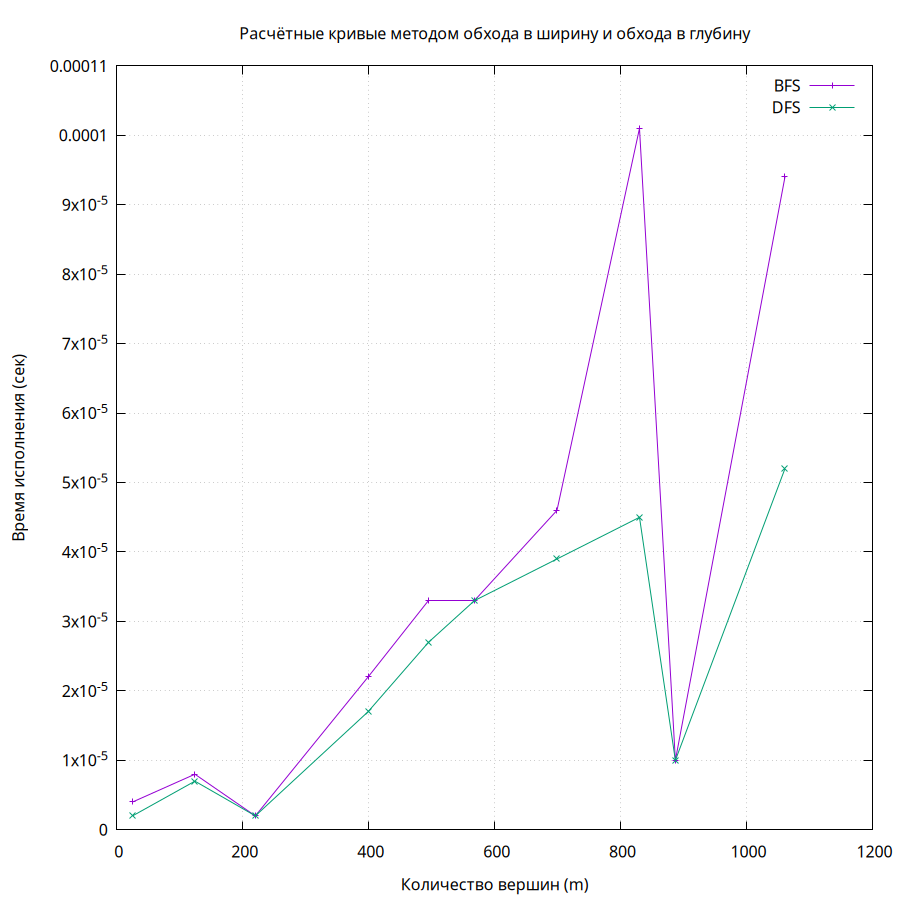
\includegraphics[width=300pt]{bfs_dfs.png}
	\end{figure}

	\begin{figure}[h]
		\centering
		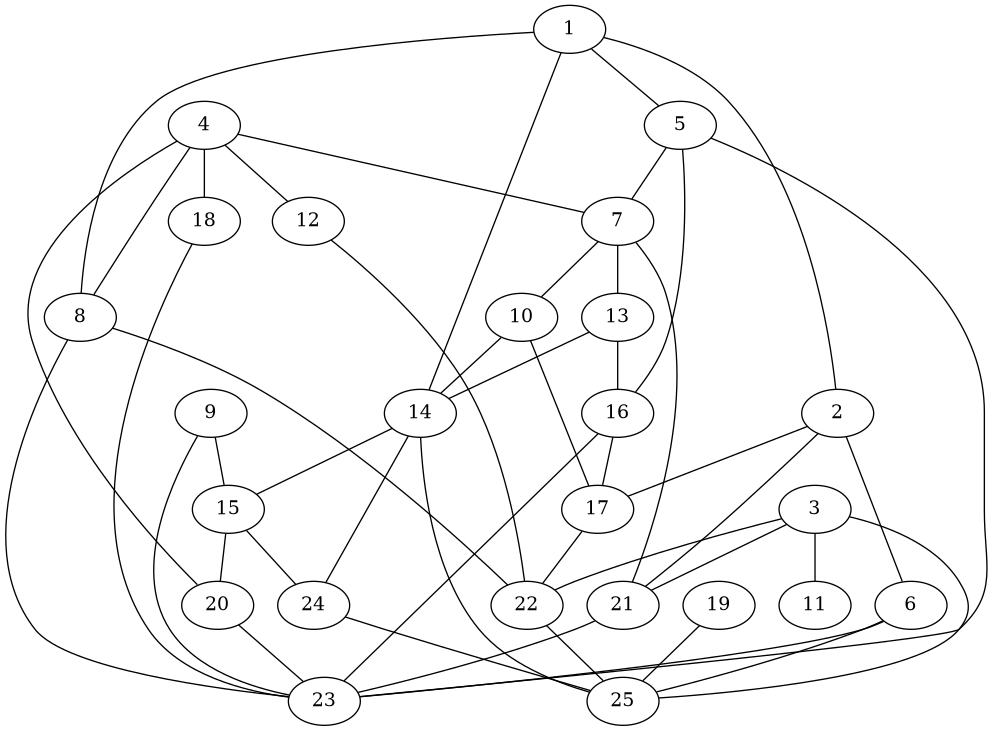
\includegraphics[width=1\textwidth]{graph_1.png}
		\caption{Граф 1.}
	\end{figure}
	\begin{figure}[h]
		\centering
		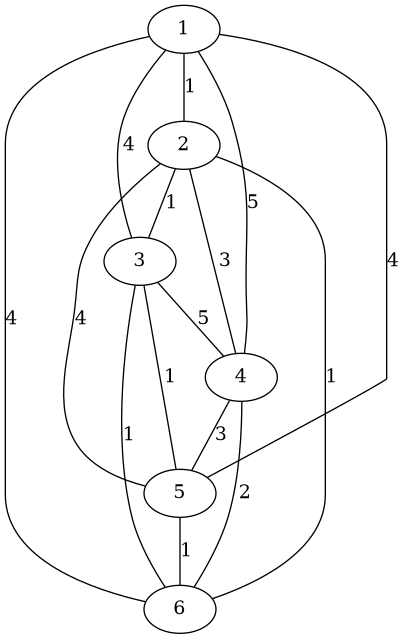
\includegraphics[width=1\textwidth]{graph_2.png}
		\caption{Граф 2.}
	\end{figure}
	\begin{figure}[h]
		\centering
		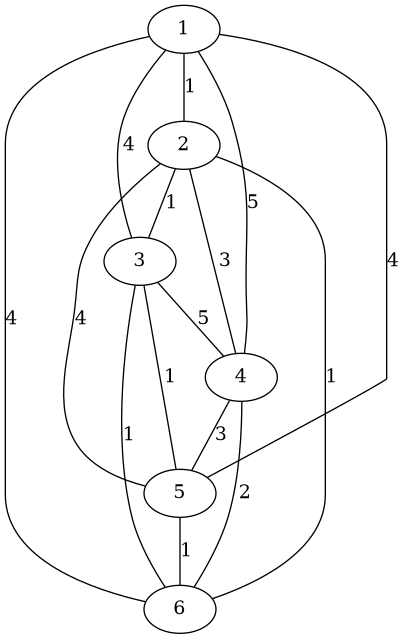
\includegraphics[width=1\textwidth]{graph_3.png}
		\caption{Граф 3.}
	\end{figure}
	\begin{figure}[h]
		\centering
		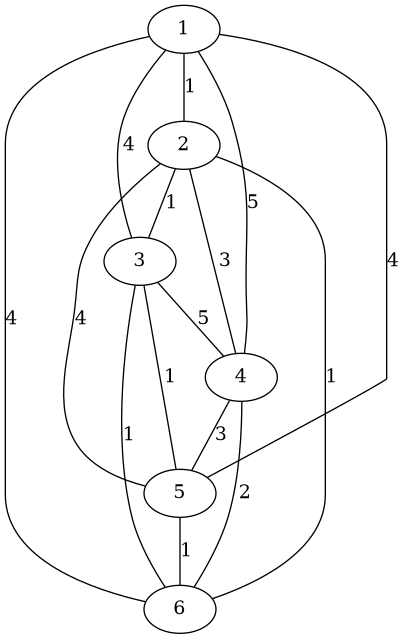
\includegraphics[width=1\textwidth]{graph_4.png}
		\caption{Граф 4.}
	\end{figure}
	\begin{figure}[h]
		\centering
		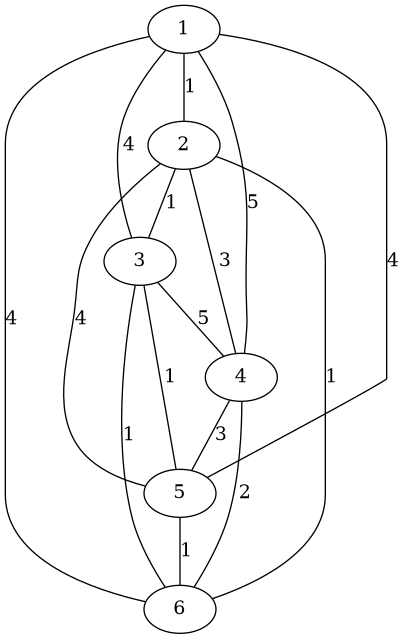
\includegraphics[width=1\textwidth]{graph_5.png}
		\caption{Граф 5.}
	\end{figure}

	\vfill
	\clearpage

	\section*{Выводы}
	\addcontentsline{toc}{section}{Выводы}

\end{document}
